% Appendix A

\chapter{Supplementary Material for \cref{selective_alignment}} % Main appendix title
\label{appendix-selal}

\section{Materials and Methods}

\subsection{Data and reference}
\label{subsec:meth_accessions}

The GENCODE v29 Human reference from
\url{https://www.gencodegenes.org/human/release_29.html} was used for all
experiments involving (simulated or experimental) human reads. The mouse
reference genome was obtained from
\url{ftp://ftp.ensembl.org/pub/release-91/fasta/mus_musculus/dna/Mus_musculus.GRCm38.dna.toplevel.fa.gz}
and the GTF was obtained from
\url{ftp://ftp.ensembl.org/pub/release-91/gtf/mus_musculus/Mus_musculus.GRCm38.91.gtf.gz}.
The VCF files for the SNPs and indels were obtained from
\url{ftp://ftp-mouse.sanger.ac.uk/REL-1410-SNPs_Indels/mgp.v4.snps.dbSNP.vcf.gz}
and
\url{ftp://ftp-mouse.sanger.ac.uk/REL-1410-SNPs_Indels/mgp.v4.indels.dbSNP.vcf.gz}
respectively. The list of 109 SRR, scripts to simulate synthetic reads, and the fasta
and true abundance files for 10 replicates of simulated data (gencode for human
and PWK for mouse) can be found at
\url{https://doi.org/10.5281/zenodo.3523437}.

\subsection{Decoy sequences}
\label{subsec:meth_decoy}

Alignment against the genome and transcriptome both have their advantages and
disadvantages, as discussed earlier. To avoid aligning genomic reads against
the transcriptome, without the need to index the complete genome, requires
finding regions with high sequence similarity between them. To obtain similar
sequences within a reference, we mapped the spliced transcript sequences against
a version of the genome where all exon segments were hard-masked (i.e.\@
replaced with \texttt{N}). We performed this mapping using
MashMap~\cite{jain2018fast}, with a segment size 500 and minimum percent
identity of 80\%. The sequence similar regions were merged (per-chromosome)
using BedTools~\cite{quinlan2010bedtools} and concatenated, giving a decoy
sequence for each chromosome. These decoys were then included during the
\salmon indexing phase, as described below. A script to obtain these decoy
sequences for any reference, given the genome, transcriptome, and annotation
is available at: \url{https://github.com/COMBINE-lab/SalmonTools/blob/master/scripts/generateDecoyTranscriptome.sh}.

\subsection{Selective alignment}
\label{subsec:meth_sa}

Selective alignment is based on the pufferfish indexing data structure first
described in~\cite{pufferfish}. Moreover, the index is augmented with the
relevant decoy sequence (either restricted decoy sequence as described
in~\Cref{subsec:meth_decoy} or the entire genome) which is marked during
indexing and handled in a special manner during alignment scoring.


The mapping approach works in 5 distinct phases (for paired-end reads).
First, exact matches between the read and transcriptome are collected.
Second, the set of transcripts to be considered for further processing are
extracted. Third, exact match chaining and chain scoring, using the algorithm
of~\citet{minimap2}, is used to determine the relevant putative mapping loci
for the read. Fourth (for paired-end reads), the mappings for the first and
second read of the pair are matched to determine the mapping loci for the
whole fragment. Finally, the computed mapping loci are scored using extension
alignment scoring~\citep{minimap2,suzuki2018introducing} before, after and 
between the exact matches belonging to the highest-scoring chain for each 
mapping. In this final step, information about the decoy sequences is used to
determine which mappings are considered valid and which are not (details are
provided below).

In the first phase of the mapping algorithm, uni-MEMs~\cite{debga} are
collected between the sequenced fragment (with each read end treated
separately) and the index. The uni-MEMs are found via k-mer lookup, and then
are extended maximally until the end of a unitig is encountered, the
end of the read is encountered, or a mismatch is encountered.  If uni-MEM 
extension terminates because it reaches the end of a unitig or because of a 
mismatch, search advances in the read and subsequent k-mers are queried in 
the index to collect other uni-MEMs shared between the read and the index.
This process is repeated until the end of the read, and results in a collection 
of uni-MEMs --- matches between the read and the index that can be efficiently 
decoded into the implied matches between the read and the reference.

In the second phase, uni-MEMs are projected to their corresponded reference
loci, and the exact matches are collated by reference and orientation. Let
$M$ denote the number of matches for the transcript, orientation pair with
the maximum number of matches for the current read. An optional
(user-determined) filtering policy is applied, whereby any transcript and
orientation pair that does not have at least $\tau M$ matches is
discarded from further consideration. The value of $\tau$ is a user-specified
fraction, set as $0.65$ by default.  This optional filtering policy, termed 
as ``filtering before chaining'', is disabled by default, but can be enabled 
via the command-line option \texttt{--hitFilterPolicy BEFORE}. Note that it
was not enabled in our experiments and the default was used. 

Next, matches along each transcript, orientation pair are sorted and
compacted. This compaction is necessary since it is possible to have matches
that are directly adjacent on both the read and reference, but which were not
extracted as a single exact match during the first phase because the
underlying uni-MEM terminated. This compaction phase eliminates such
fragmentation due to uni-MEM termination, and reduces the number of exact
matches that must be considered by the chaining algorithm. Candidate mapping
locations are determined by applying the chaining algorithm of
minimap2~\cite{minimap2} to the exact matches for each transcript passing the
previous filter. If multiple equally-good positions for a read along a
transcript, in terms of their chaining score, are discovered, they are all
propagated downstream in the mapping procedure until mappings for paired-end
reads are merged. Likewise, if a read is determined to map to a transcript in
both the forward and reverse-complement orientation, then all equally-best
mapping loci in both orientations are propagated downstream in the mapping
procedure.  Let $S$ be the best chaining score obtained for any mapping of
the current read.  An optional filter is applied where any mapping with a 
chaining score less than $\tau' S$ is discarded from further consideration.
By default, this filter, termed as ``fitering after chaining'', is enabled 
by default and $\tau'$ is set as 0.65.

For paired-end reads, the pairs are merged by determining, for each
transcript, the locations of the read ends that respect the expected mapping
constraints (e.g. that the leftmost position of the reverse complement read
is to the right of the leftmost position of the forward-strand read, and the
distances between the reads is less than the maximum allowed insert size). If
passed the appropriate flag \texttt{--allowDovetails}, then
dovetailed~\cite{bt2manual} mappings are allowed, but they are prioritized
below any non-dovetailed mapping.


All putative mappings are scored using the ksw2~\cite{minimap2,suzuki2018introducing} library
for alignment extension. We note that we compute only the optimal alignment
score, and not the details of the alignment itself (i.e.\@ the CIGAR string),
which improves the speed of this mapping validation. To avoid redundant
computation of the same alignment problem (which is quite prevalent when mapping
directly to the transcriptome, as many alignments to alternatively-spliced
transcripts will be identical), \hsa maintains a per-read alignment cache. This
alignment cache is a hash table where the key is a hash of the reference
transcriptome substring where the read is predicted to align, and the value is
the previous alignment score computed for such a substring. Thus, if multiple
transcripts would produce identical alignments for the same read, because the
read maps to identical regions of these transcripts, \hsa is able to avoid
this redundant work.

Finally, all of the relevant alignments are grouped by their associated
alignments scores. Any alignments that fall below the (user-provided) threshold
(default of $0.65$ of the maximum obtainable alignment score) for a minimum
valid alignment score are discarded. During alignment scoring, the score of the
best alignment for a given fragment to any decoy sequence as well as to any
non-decoy sequence is computed and stored. If the best alignment score to a
decoy sequence is strictly greater than the best alignment score to a non-decoy
sequence, then all of the fragment's mappings are considered invalid and the
fragment is not considered for quantification. Otherwise, any alignments to
decoy sequences are filtered out, and the remaining alignments to valid
transcripts are further processed by \salmon using range-factorized equivalence
classes~\cite{ddfact}, which allows the relevant information about the scores
for the different alignments of the read to be appropriately summarized and used
for quantification.

\subsection{Analysis details}
\label{subsec:notes}

\paragraph{A note on the difference between \hsa and \saf}
This manuscript introduces the idea of selective alignment over a reference sequence 
indexed using the pufferfish~\cite{pufferfish} data structure, implemented in the \salmon program. The index
takes as input a set of decoy sequences, which are not part of the reference transcriptome 
and are, therefore, not quantified. In our analyses, we considered the performance of the selective alignment 
algorithm when paired with two different sets of decoys as input. In the first approach, referred to as \hsa in the manuscript, 
the index is built on the transcriptome and regions of the genome that
have high sequence similarity with the transcriptome. In the second approach, referred to as \saf, 
the complete genome is included in the pufferfish index as a set of decoys. Hence, the 
index for \hsa contains a smaller portion of the genome, whereas the \saf index contains
the full genome. Also, note that selective alignment replaces the \qm algorithm previously 
used in the \salmon program.

\paragraph{A note on on orphan and dovetail mappings}
We attempted to normalize for some mapping-related differences between
methods that have little to do with the ability of the aligner to appropriately
find the correct loci for a read, and instead have to do with constraints placed
on what constitutes a valid mapping. Specifically, when projecting to the
transcriptome, STAR disallows orphan mappings (cases where one end of a fragment
aligns to a transcript but the other end does not). Likewise it is recommended
practice in existing alignment-based quantification tools~\citep{rsem,hensman2015fast,glaus2012identifying},
when using Bowtie2, to discard discordant and orphaned alignments. Thus, in our
analyses, we disallowed orphaned mappings so that, in paired-end datasets, the
pair is discarded if only one end of a fragment is mapped, or if the fragment
ends only map to distinct transcripts. To be consistent with the default
behavior of Bowtie2, the configurations of \qm and \hsa were also set to disallow dovetailed mappings (mappings where the
first mapped base of the reverse complement strand read is upstream of the first
mapped base of the forward strand read). While Bowtie2's scoring function (when performing global alignment) 
does not allow insertions or deletions to occur at the beginning or end of the read, we attempted to minimize the 
effect of this structural constraint on alignments by setting the \texttt{--gbar} parameter to 1.

\paragraph{A note on genomic alignment, as used in this manuscript.}
We explored differences that arise between quantification
based on alignment of the sequencing reads to the genome and the transcriptome. 
We considered genomic alignment here to be the process of
alignment to the genome --- with the benefit of a known annotation ---
with subsequent projection to the transcriptome. That is, genomic
alignment is characterized based on running STAR (with appropriate parameters)
to align the reads to the genome, and then making use of the
transcriptomically-projected alignments output by STAR via the
\texttt{--quantMode TranscriptomeSAM} flag (as would be used in e.g.\@ a
STAR\citep{star}/RSEM\citep{rsem}-based quantification pipeline). Such an
approach is necessarily concerned only with how well STAR is able to align the
sequenced reads to the annotated transcriptome of the organism being
assayed, and our assessment is concerned only with the accuracy of
quantification of known and annotated isoforms. Importantly, spliced alignment of
RNA-seq reads to the genome can be a useful tool in tackling a broader range of
problems and in a larger set of cases than can unspliced alignment to a known
transcriptome. For example, spliced alignment of sequencing reads to the genome
can be done in the absence of an annotation of known isoforms, and can be used
to help identify novel exons, isoforms, or transcribed regions of the genome,
while unspliced alignment to a pre-specified set of transcripts does not admit
this type of analysis. Further, alignment directly to the genome can easily cope
with events like intron retention, which are more difficult to account for when
using methods that align reads to the transcriptome.

\paragraph{A note on the influence of short transcripts on quantification.} 
The human GENCODE v29 reference includes transcripts as short as 8bp, which is
much shorter than a single sequencing read or the typical fragment length in
most RNA-seq experiments. While RNA-seq might not be the appropriate method to
quantify these transcripts, depending on the alignment method, they may have
mapped reads and obtain non-zero expression values. In our analyses, we observed
that lightweight mapping methods that do not perform end-to-end alignment tend
to assign reads to shorter transcripts when there is an exact match. This effect
has been explored in some detail by~\citet{wu2018limitations}. In such a
scenario, it is hard to judge the true origin of the read, and while this may
lead to some differences between mapping and alignment-based methods, we showed that the
differences in quantification estimates for short transcripts account for only a
very small fraction of the overall differences between methods. 
Since it is difficult to judge how these shorter transcripts, and the
reads aligning to them, should be handled, we simply highlighted this issue and
refrained from suggesting a particular strategy or attempting to determine which
method performed better or worse on transcripts shorter than $300$bp. 

\subsection{Tools}
\label{subsec:commands}
We used \salmon v0.15.0 for quasi-mapping and \salmon v1.0 for \hsa and \saf, Bowtie2 version 2.3.4.3, STAR version 2.6.1b, tximport
version 1.12.3, DESeq2 version 1.24.0, kallisto version 0.45.1, edgeR version 3.24.3, limma version 3.38.3, 
RSEM version 1.2.28, Trim Galore version 0.5.0, bedtools v2.28.0, sleuth version 0.30.0 and
MashMap v2.0. All simulated datasets were generated using Polyester version 1.18.0.

For quality trimming the reads we used the following command:
\raggedright
\begin{enumerate}
\item \textbf{trim\_galore} \texttt{-q 20 --phred33 --length 20 --paired <fastq file>}
\end{enumerate}

For indexing, we use the following extra command line arguments, along with the regular
indexing and threads parameters:
\begin{enumerate}
\item \textbf{STAR} \texttt{--genomeFastaFiles <fasta file> --sjdbGTFfile <gtf file> --sjdbOverhang 100}
\item \textbf{Bowtie2} \texttt{default}
\item \textbf{salmon} \texttt{-k 23 --keepDuplicates}
\item \textbf{kallisto} \texttt{-k 23}
\end{enumerate}

For quantification, we use the following extra command line, along with regular
index and threads, with each tools we compare against:
\raggedright
\begin{enumerate}
	\item \textbf{SA and SAF} \texttt{--mimicBT2 --useEM}
	\item \textbf{quasi} \texttt{--rangeFactorizationBins 4 --discardOrphansQuasi --useEM --noSA}
	\item \textbf{Bowtie2} \texttt{--sensitive -k 200 -X 1000 --no-discordant --no-mixed --gbar 1}
	\item \textbf{Bowtie2\_strict} \texttt{--sensitive --dpad 0 --gbar 99999999 --mp 1,1
	  --np 1 --score-min L,0,-0.1 --no-mixed --no-discordant -k 200 -I 1 -X 1000}
	\item \textbf{Bowtie2\_RSEM} \texttt{--sensitive --dpad 0 --gbar 99999999 --mp 1,1
	  --np 1 --score-min L,0,-0.1 --no-mixed --no-discordant -k 200 -I 1 -X 1000}
	\item \textbf{STAR} \texttt{--outFilterType BySJout --alignSJoverhangMin 8 
	--outFilterMultimapNmax 20 --alignSJDBoverhangMin 1 --outFilterMismatchNmax 999
	--outFilterMismatchNoverReadLmax 0.04 --alignIntronMin 20 --alignIntronMax 1000000 
	--alignMatesGapMax 1000000 --readFilesCommand zcat --outSAMtype BAM Unsorted 
	--quantMode TranscriptomeSAM --outSAMattributes NH HI AS NM MD 
	--quantTranscriptomeBan Singleend}
	\item \textbf{STAR\_strict} \texttt{--outFilterType BySJout --alignSJoverhangMin 8 
	--outFilterMultimapNmax 20 --alignSJDBoverhangMin 1 --outFilterMismatchNmax 999
	--outFilterMismatchNoverReadLmax 0.04 --alignIntronMin 20 --alignIntronMax 1000000 
	--alignMatesGapMax 1000000 --readFilesCommand zcat --outSAMtype BAM Unsorted 
	--quantMode TranscriptomeSAM --outSAMattributes NH HI AS NM MD
	--quantTranscriptomeBan IndelSoftclipSingleend}
	\item \textbf{STAR\_RSEM} \texttt{--outFilterType BySJout --alignSJoverhangMin 8 
	--outFilterMultimapNmax 20 --alignSJDBoverhangMin 1 --outFilterMismatchNmax 999
	--outFilterMismatchNoverReadLmax 0.04 --alignIntronMin 20 --alignIntronMax 1000000 
	--alignMatesGapMax 1000000 --readFilesCommand zcat --outSAMtype BAM Unsorted 
	--quantMode TranscriptomeSAM --outSAMattributes NH HI AS NM MD
	--quantTranscriptomeBan IndelSoftclipSingleend}
	\item \textbf{RSEM} \texttt{default}
	\item \textbf{kallisto} \texttt{default} or \texttt{--rf-stranded} as appropriate
\end{enumerate}

\begin{table}[h!]
 \centering
 \begin{tabular}{cccccc}
   \hline
   				& \multicolumn{1}{p{1.5cm}}{\centering Genome indexed} & \multicolumn{1}{p{1.5cm}}{\centering Alignment scoring} &
				\multicolumn{1}{p{1.5cm}}{\centering Indels allowed} & \multicolumn{1}{p{2cm}}{\centering End-to-end alignment} &
				\multicolumn{1}{p{2cm}}{\centering Quantification method} \\ \hline
      Bowtie2		& \xmark & \cmark & \cmark & \cmark & \salmon \\
      Bowtie2\_strict	& \xmark & \cmark & \xmark & \cmark & \salmon \\
      Bowtie2\_RSEM	& \xmark & \cmark & \xmark & \cmark & RSEM \\
      STAR			& \cmark & \cmark & \cmark & \cmark & \salmon \\
      STAR\_strict	& \cmark & \cmark & \xmark & \cmark & \salmon \\
      STAR\_RSEM	& \cmark & \cmark & \xmark & \cmark & RSEM \\
      quasi			& \xmark & \xmark & \cmark & \xmark & \salmon \\
      \hsa			& \xmark$^{*}$ & \cmark$^{**}$ & \cmark & \xmark & \salmon \\
      \saf			& \cmark & \cmark$^{**}$ & \cmark & \xmark & \salmon \\
   \hline
\end{tabular}
 \caption{Various factors altered under each pipeline. *Here, under \hsa, only
  regions of the genome that are sequence similar to the transcriptome are indexed, but not
  the whole genome. Refer to~\Cref{subsec:meth_decoy} for further details on how the sequences are obtained.
  **While \hsa and \saf produce alignment scores, they do not perform backtracing or reconstruct the edit
  operations that were used to obtain the optimal alignment score.}
 \label{tab:methods}
\end{table}

\begin{figure}[h!]
  \centering
  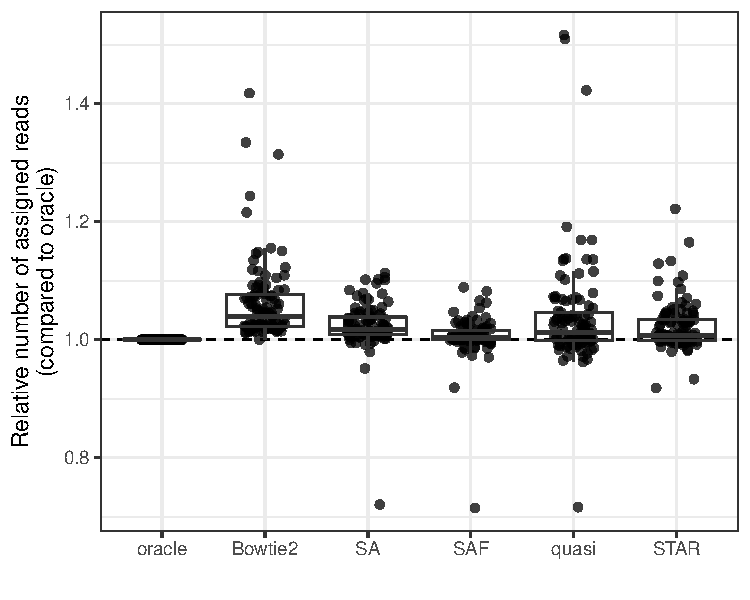
\includegraphics[width=\linewidth]{selal/mrate.pdf}
  \caption{Mapping rates of different methods, relative to oracle, for 109 experimental samples.}
  \label{fig:mrate}
\end{figure}

\begin{table}[h!]
 \centering
 \begin{tabular}{ccccccc}
   \hline
         & Oracle & Bowtie2 & SAF & \hsa & quasi & STAR\\ \hline
 Oracle & 1.000/0.000 & $\numprint{0.858495}$/$\numprint{0.053736}$ & $\numprint{0.919992}$/$\numprint{0.028552}$ & $\numprint{0.873352}$/$\numprint{0.045867}$& $\numprint{0.843022}$/$\numprint{0.053193}$& $\numprint{0.889439}$/$\numprint{0.039311}$\\
 Bowtie2 & -- & 1.000/0.000 & $\numprint{0.817429}$/$\numprint{0.063481}$ & $\numprint{0.863387}$/$\numprint{0.038621}$ & $\numprint{0.783076}$/$\numprint{0.067582}$ & $\numprint{0.790747}$/$\numprint{0.068541}$ \\
 SAF & -- & -- & 1.000/0.000 & $\numprint{0.906522}$/$\numprint{0.052332}$ & $\numprint{0.864903}$/$\numprint{0.049687}$ & $\numprint{0.909014}$/$\numprint{0.023030}$\\
 \hsa & -- & -- & -- & 1.000/0.000 & $\numprint{0.829317}$/$\numprint{0.063462}$ & $\numprint{0.836573}$/$\numprint{0.058815}$ \\
 quasi &  -- & --  & -- & -- & 1.000/0.000 & $\numprint{0.858436}$/$\numprint{0.052212}$\\
 STAR &  -- & --  & -- & -- & -- & 1.000/0.000 \\
 \hline
\end{tabular}
 \caption{Mean/standard deviation of Spearman correlation between all methods on $40$ single-cell experimental datasets after 
 removing short transcripts with length $<300$. }
 \label{tab:withoutshortsc}
\end{table}

\begin{table}[h!]
 \centering
 \begin{tabular}{ccccccc}
   \hline
         & Oracle & Bowtie2 & SAF & \hsa & quasi & STAR\\ \hline
 Oracle & 1.000/0.000 & $\numprint{0.949207}$/$\numprint{0.022744}$ & $\numprint{0.970706}$/$\numprint{0.008334}$ & $\numprint{0.954241}$/$\numprint{0.013979}$& $\numprint{0.907292}$/$\numprint{0.031031}$& $\numprint{0.962499}$/$\numprint{0.012450}$\\
 Bowtie2 & -- & 1.000/0.000 & $\numprint{0.940024}$/$\numprint{0.026027}$ & $\numprint{0.961004}$/$\numprint{0.017293}$ & $\numprint{0.901297}$/$\numprint{0.034042}$ & $\numprint{0.919557}$/$\numprint{0.025325}$ \\
 SAF & -- & -- & 1.000/0.000 & $\numprint{0.971655}$/$\numprint{0.015035}$ & $\numprint{0.913026}$/$\numprint{0.030584}$ & $\numprint{0.954660}$/$\numprint{0.011279}$\\
 \hsa & -- & -- & -- & 1.000/0.000 & $\numprint{0.913908}$/$\numprint{0.028960}$ & $\numprint{0.932170}$/$\numprint{0.016787}$ \\
 quasi &  -- & --  & -- & -- & 1.000/0.000 & $\numprint{0.903269}$/$\numprint{0.029167}$\\
 STAR &  -- & --  & -- & -- & -- & 1.000/0.000 \\
 \hline
\end{tabular}
 \caption{Mean/standard deviation of Spearman correlation between all methods on $69$ bulk experimental datasets after 
 removing short transcripts with length $<300$. }
 \label{tab:withoutshortbulk}
\end{table}

\begin{figure}[h!]
    \centering
     \begin{subfigure}[t]{0.49\textwidth}
     \centering
  	  	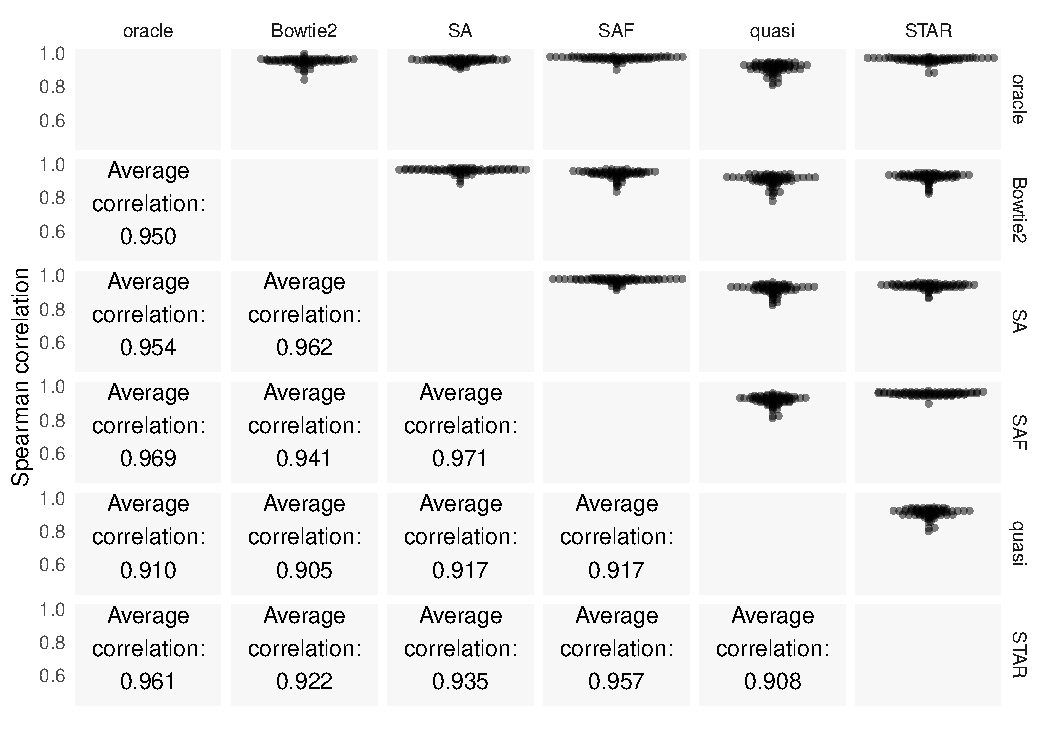
\includegraphics[width=\linewidth]{selal/bulk_pairwise_correlations_real_data_count.pdf}
		\caption{Bulk}
    \end{subfigure}
     \begin{subfigure}[t]{0.49\textwidth}
     \centering
  	  	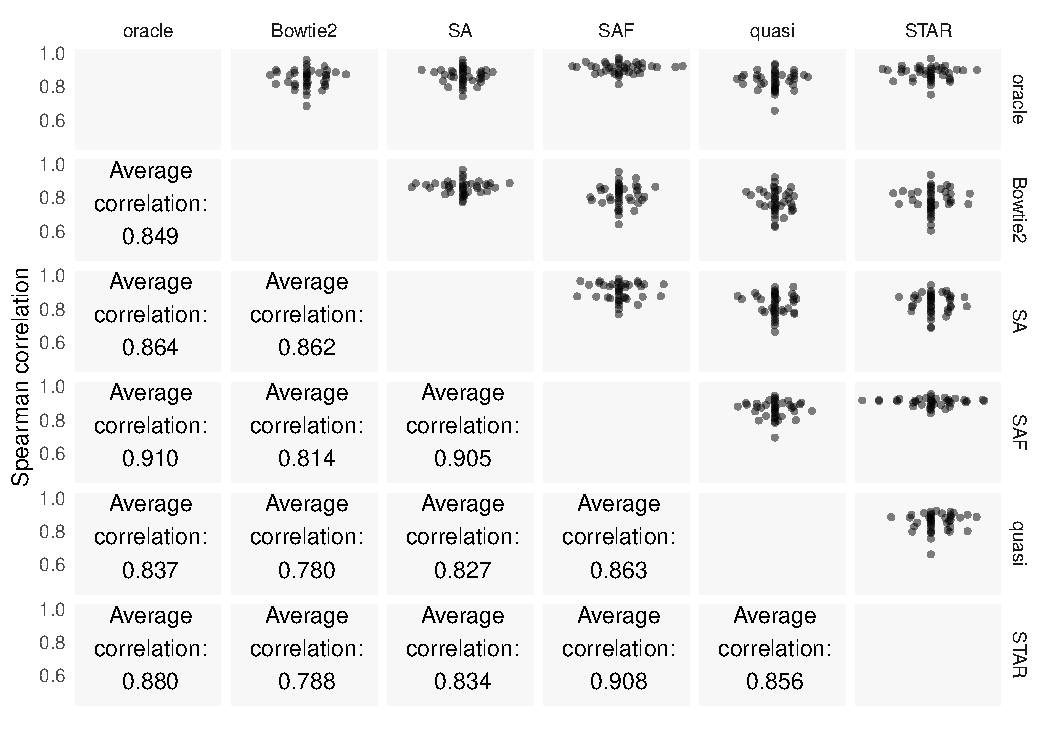
\includegraphics[width=\linewidth]{selal/singlecell_pairwise_correlations_real_data_count.pdf}
		\caption{Single-cell}
    \end{subfigure}   
     \caption{The upper triangle of the matrix shows swarm plots of pairwise correlations of read counts predicted by
       the different approaches on the experimental samples. The bottom half 
       shows the average Spearman correlations between methods across the $109$ bulk and single-cell samples.}
    \label{fig:swarmcount}
\end{figure}

\begin{figure}[h!]
    \centering
    \begin{subfigure}[t]{0.7\textwidth}
        \centering
  	  	 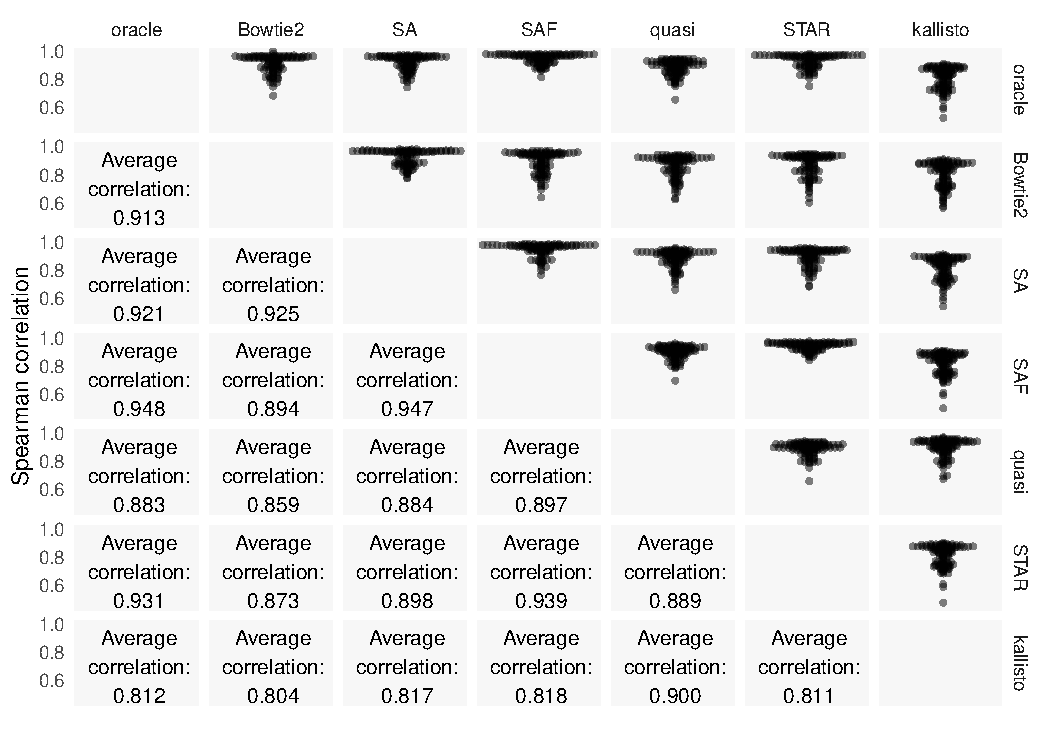
\includegraphics[width=\linewidth]{selal/pairwise_correlations_real_data_kallisto.pdf}
		\caption{}
    \end{subfigure}
    ~ 
    \begin{subfigure}[t]{0.7\textwidth}
        \centering
  	  	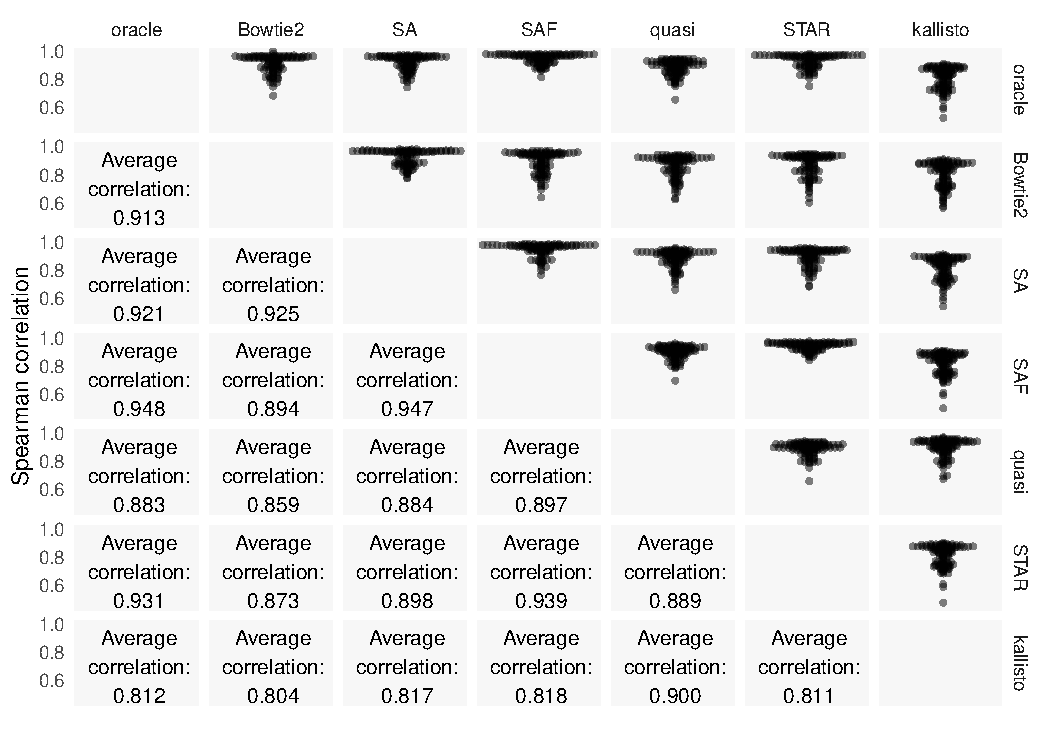
\includegraphics[width=\linewidth]{selal/pairwise_correlations_real_data_kallisto.pdf}
		\caption{}
    \end{subfigure}
    \caption{The top half of each matrix shows swarm plots of the pairwise correlations using count (a) and TPM (b) values
        predicted by the different approaches on the experimental samples. The
        bottom half shows the average Spearman correlations between methods
        across the $109$ samples. Note that the quantification method for each
        pipeline is the same, except \kallisto, where both the mapping and
        quantification algorithms are different. Hence, while other methods
        disallow orphaned reads and dovetailed mappings, the \kallisto output
        will include them, which may explain, in part, the increased divergence
        from the alignment-based methods.}
    \label{fig:kallisto}
\end{figure}

\begin{figure}[t!]
    \centering
    \begin{subfigure}[t]{0.45\textwidth}
        \centering
	    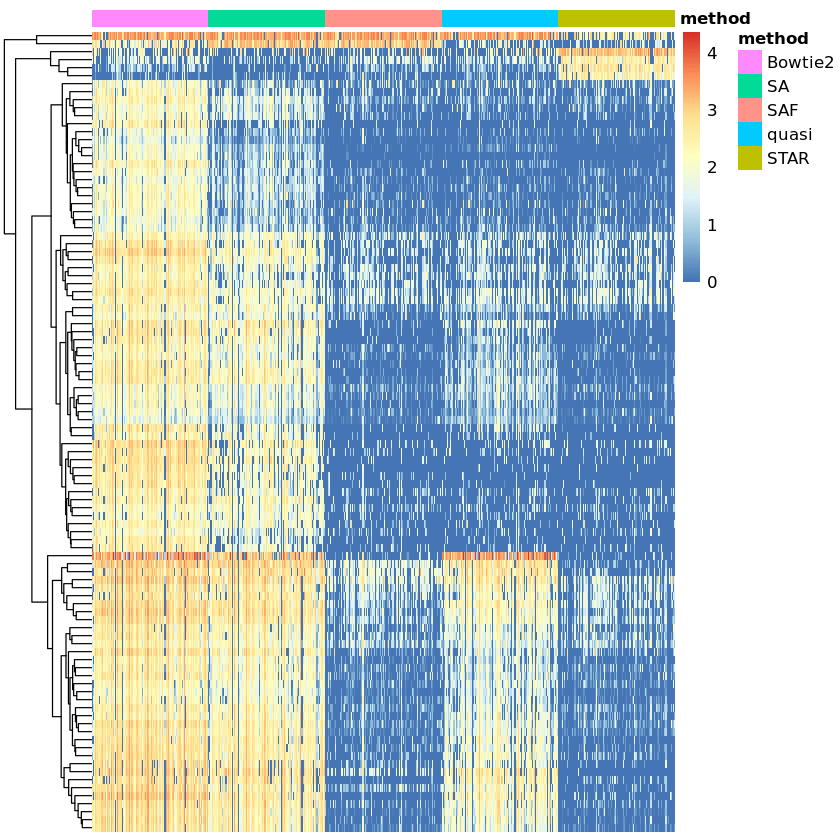
\includegraphics[width=\linewidth]{selal/heatmap_100.png}
	    \caption{}
    \end{subfigure}
    ~
    \begin{subfigure}[t]{0.45\textwidth}
        \centering
	    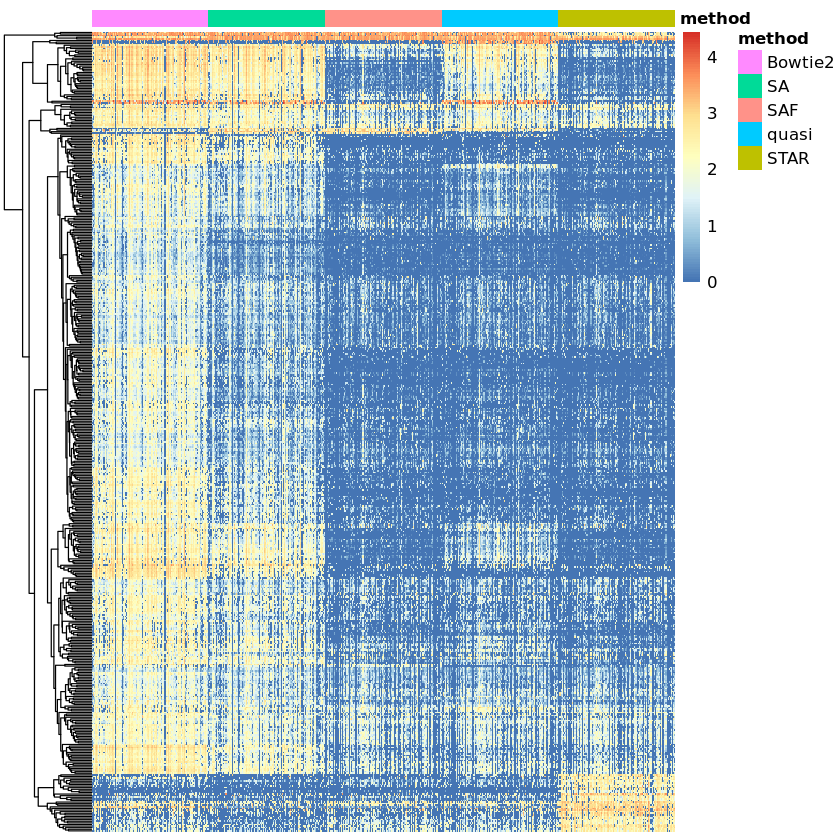
\includegraphics[width=\linewidth]{selal/heatmap_500.png}
	    \caption{}
    \end{subfigure}
    ~
     \begin{subfigure}[t]{0.45\textwidth}
     \centering
	    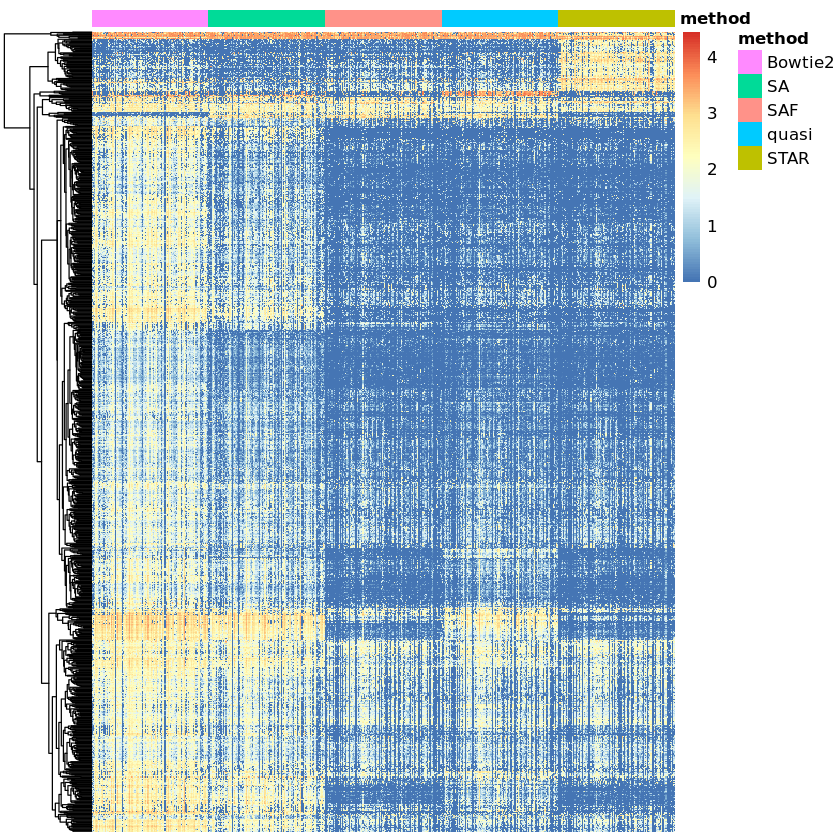
\includegraphics[width=\linewidth]{selal/heatmap_1k.png}
	    \caption{}
    \end{subfigure}
    \caption{The $\log_2(\text{CPM})$ for 109 samples grouped by
      method for the top 100 (a), 500 (b), and 1000 (c) differential transcripts. 
      Limma-trend was used with \texttt{scaledTPM} counts 
	(generating counts from per-sample TPMs by scaling to the library size) via
	tximport~\cite{soneson2015differential}, with a \texttt{prior.count} of
	3, and using a design of \texttt{$\sim$sample + method}. An F-statistic was
	generated by specifying coefficients representing differences among the methods
	and the top transcripts chosen using the F-test p-value.}
      \label{fig:heatmap}
\end{figure}

\begin{figure}[h!]
    \centering
     \begin{subfigure}[t]{0.49\textwidth}
     \centering
  	  	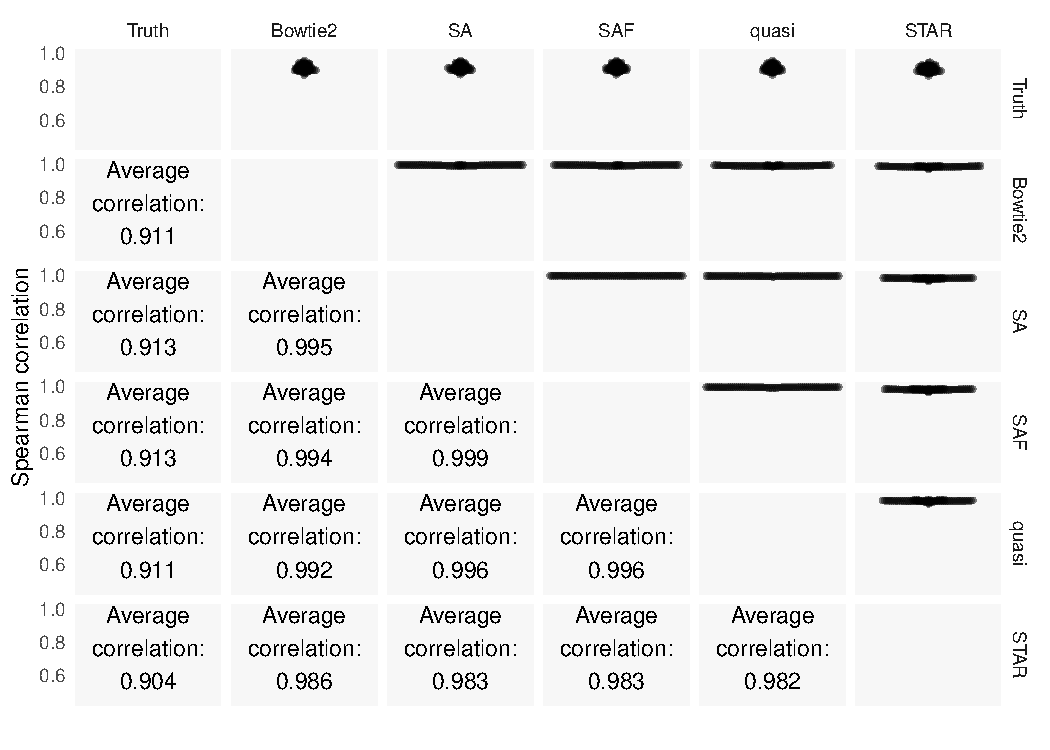
\includegraphics[width=\linewidth]{selal/bulk_pairwise_correlations_sim_data.pdf}
		\caption{Bulk}
    \end{subfigure}
     \begin{subfigure}[t]{0.49\textwidth}
     \centering
  	  	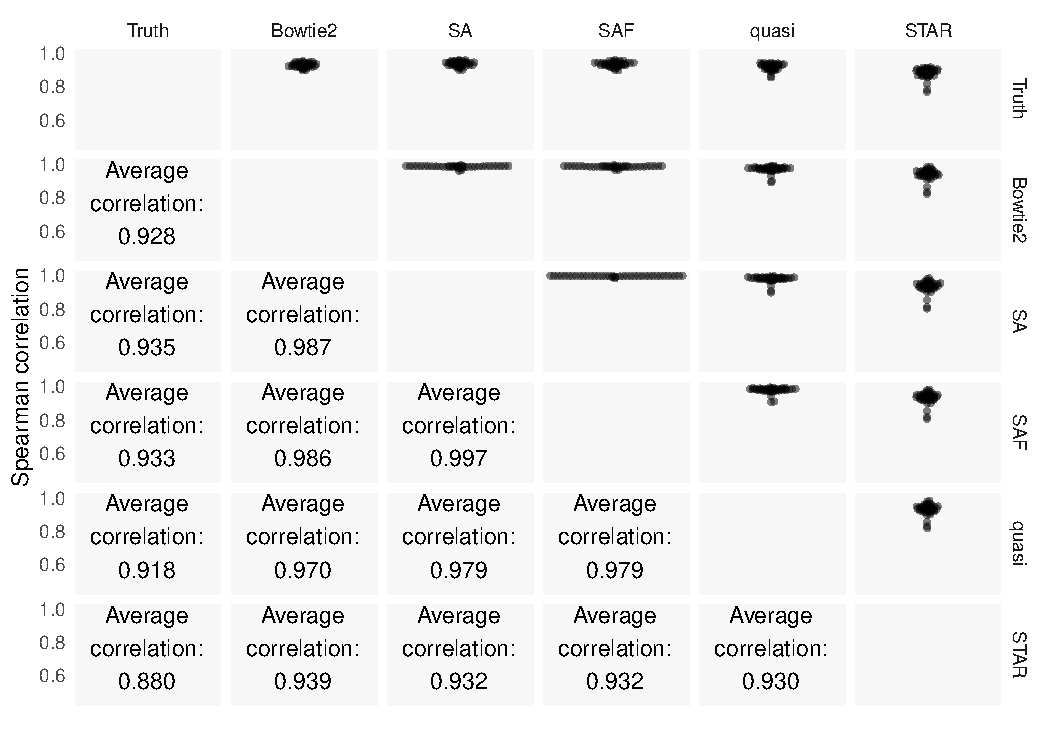
\includegraphics[width=\linewidth]{selal/singlecell_pairwise_correlations_sim_data.pdf}
		\caption{Single-cell}
    \end{subfigure}
     \caption{The top half of the matrix shows swarm plots of the pairwise correlations of TPM 
	 values predicted by the
       different approaches with each other and with the ground truth abundances
       on the simulated samples. The bottom half shows the average Spearman
       correlations between the different approaches across the $109$ samples.
       The expected effective length of each transcript was computed according
       to the true fragment length distribution. Given the true fragment counts
       and expected effective lengths, the TPM is computed as in~\citet{rsem}.}
    \label{fig:swarmsimTPM}
\end{figure}

\begin{figure}[ht!]
    \centering
    \begin{subfigure}[t]{0.49\textwidth}
        \centering
  	  	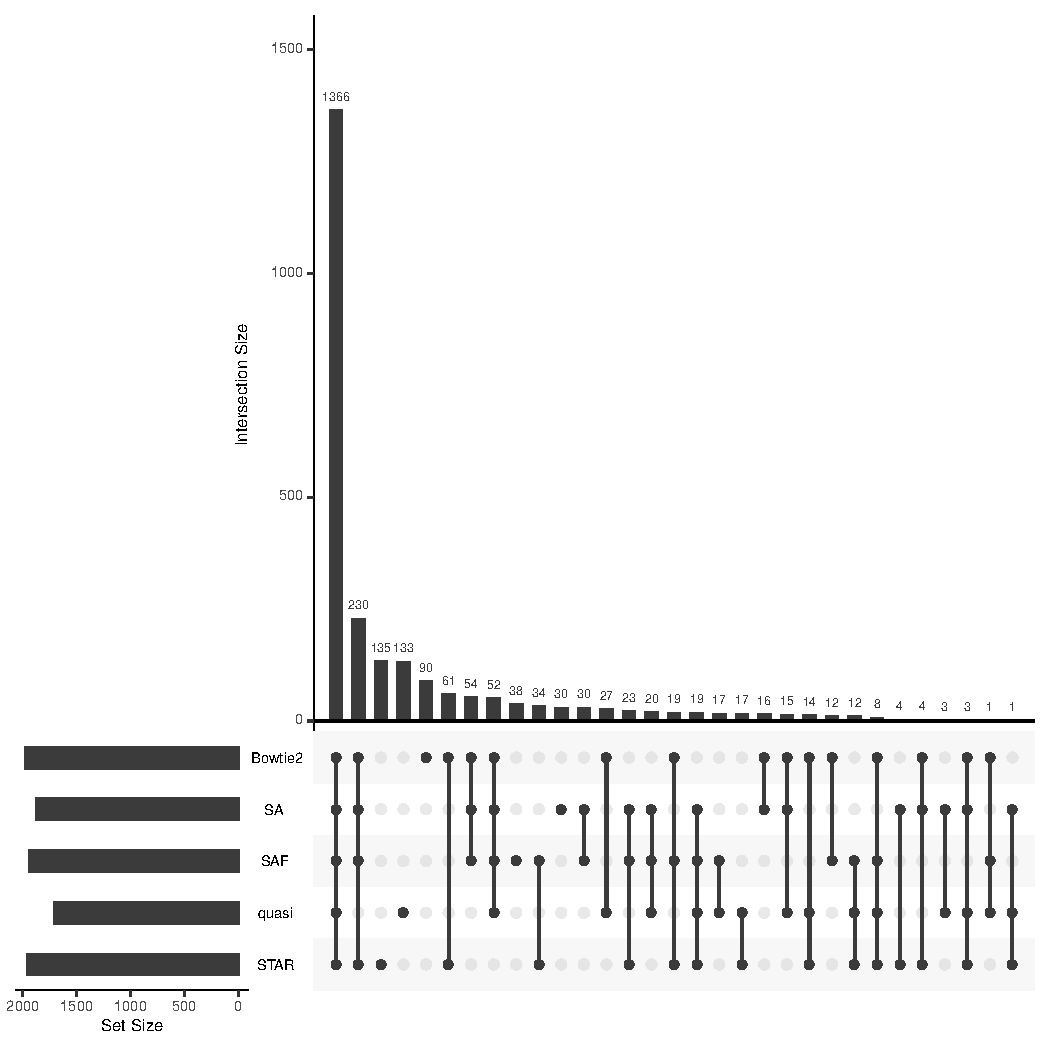
\includegraphics[width=\linewidth]{selal/alsfdr5.pdf}
		\caption{}
    \end{subfigure}
    ~ 
    \begin{subfigure}[t]{0.49\textwidth}
        \centering
  	  	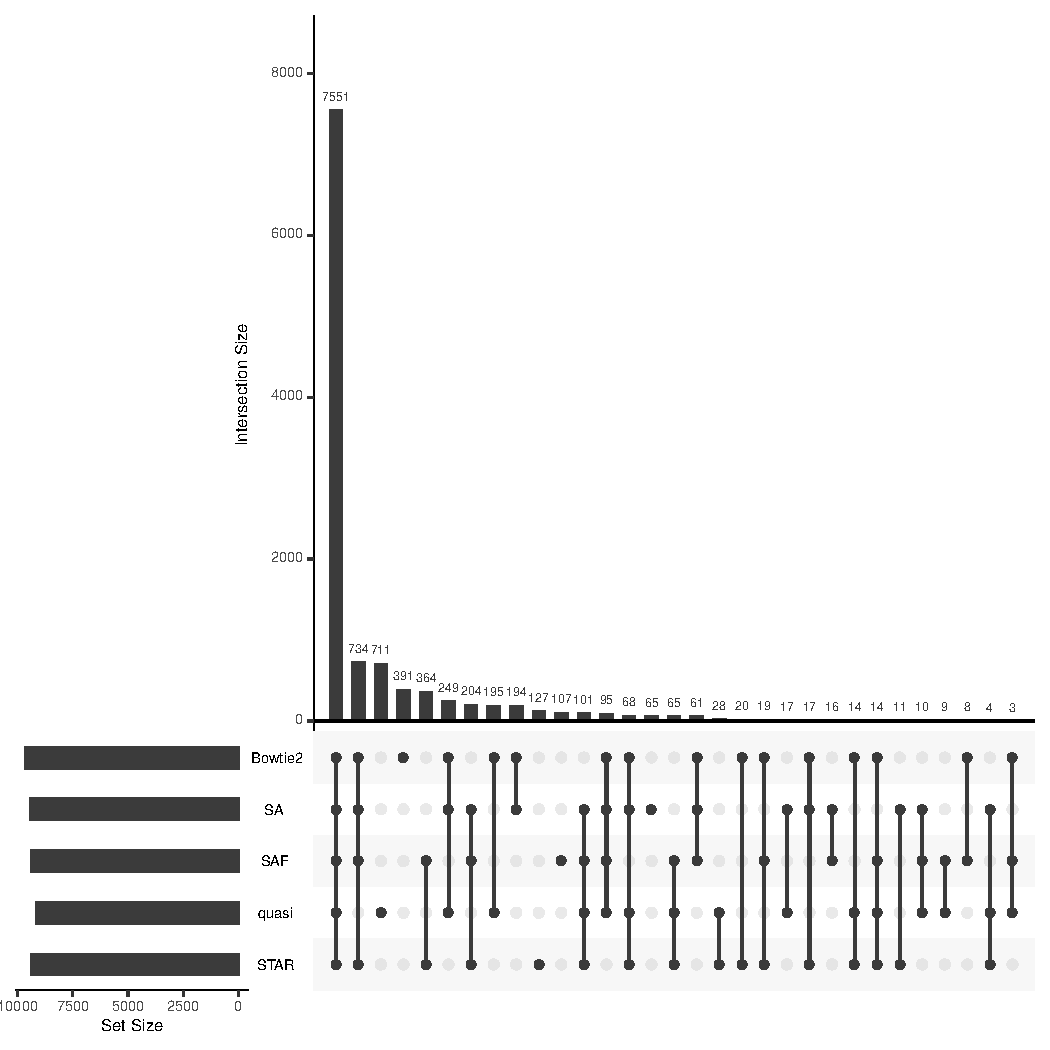
\includegraphics[width=\linewidth]{selal/hsvfdr5.pdf}
		\caption{}
    \end{subfigure}
    ~
    \begin{subfigure}[t]{0.49\textwidth}
        \centering
  	  	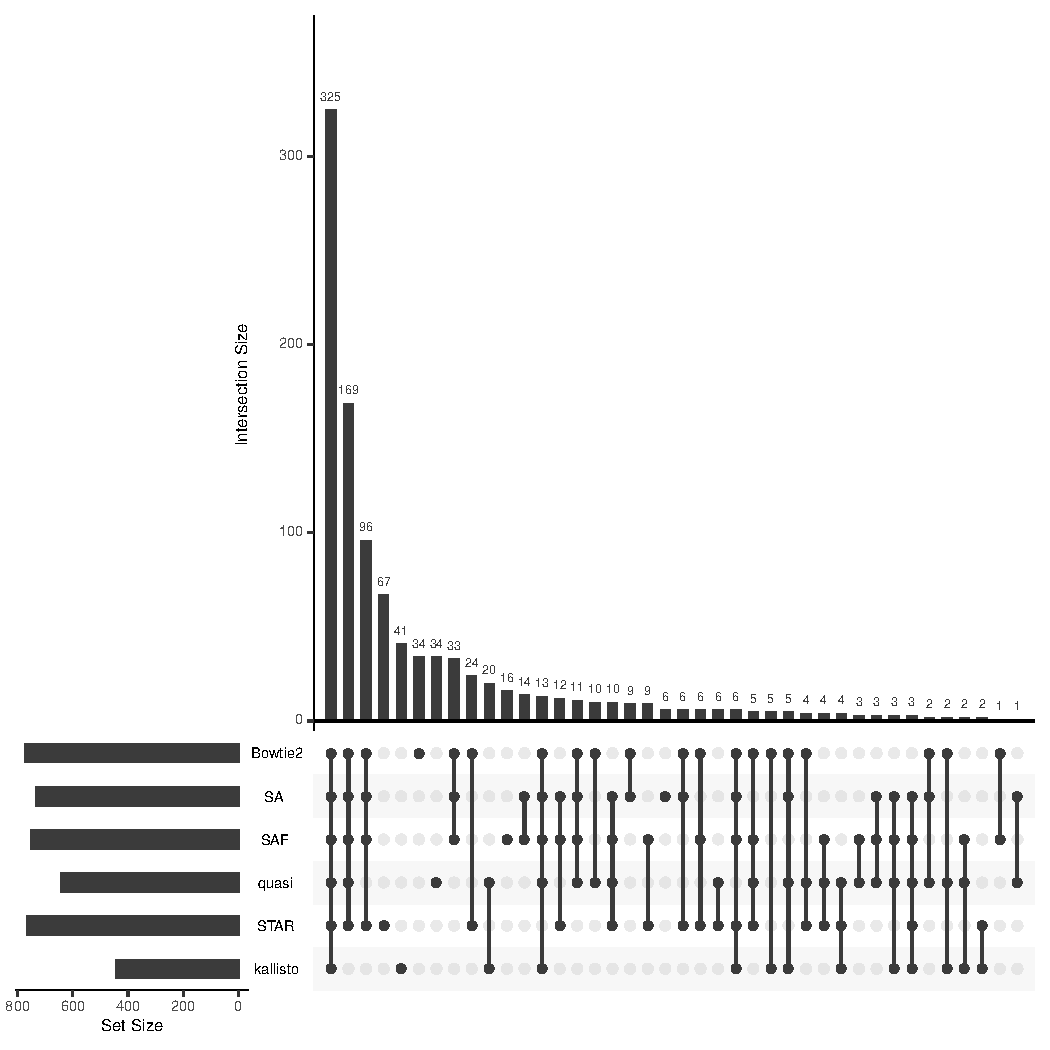
\includegraphics[width=\linewidth]{selal/alskal.pdf}
		\caption{}
    \end{subfigure}
    ~ 
    \begin{subfigure}[t]{0.49\textwidth}
        \centering
  	  	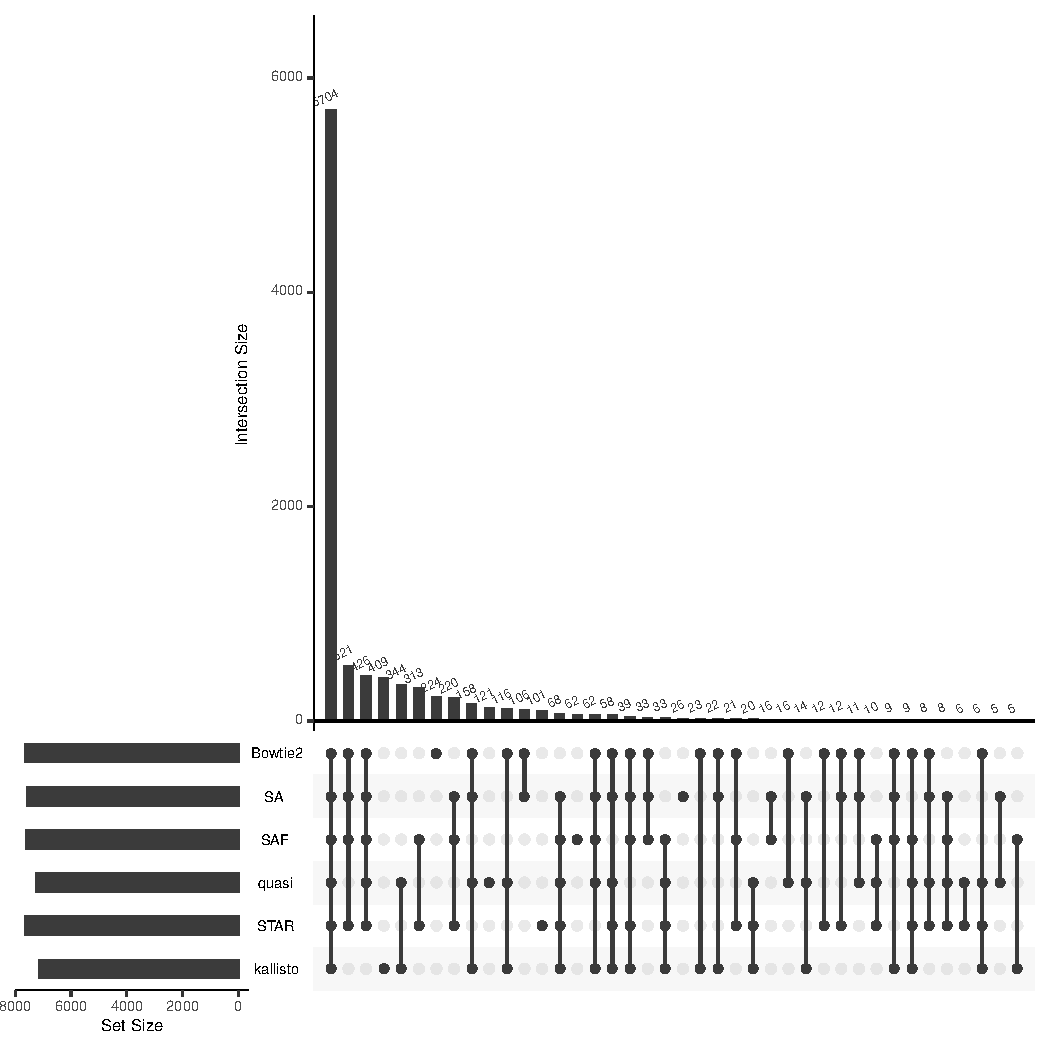
\includegraphics[width=\linewidth]{selal/hsvkal.pdf}
		\caption{}
    \end{subfigure}
    \caption{Comparison of sets of differentially expressed genes, and their overlaps, computed using each method.
    Figures (a) and (b) shows the results for the two datasets when filtered at an FDR of $0.05$ and 
    (c) and (d) shows the results at FDR $0.01$ after including kallisto as an additional lightweight mapping approach.}
    \label{fig:suppdge}
\end{figure}

\begin{figure}[ht!]
    \centering
    \begin{subfigure}[t]{0.49\textwidth}
        \centering
  	  	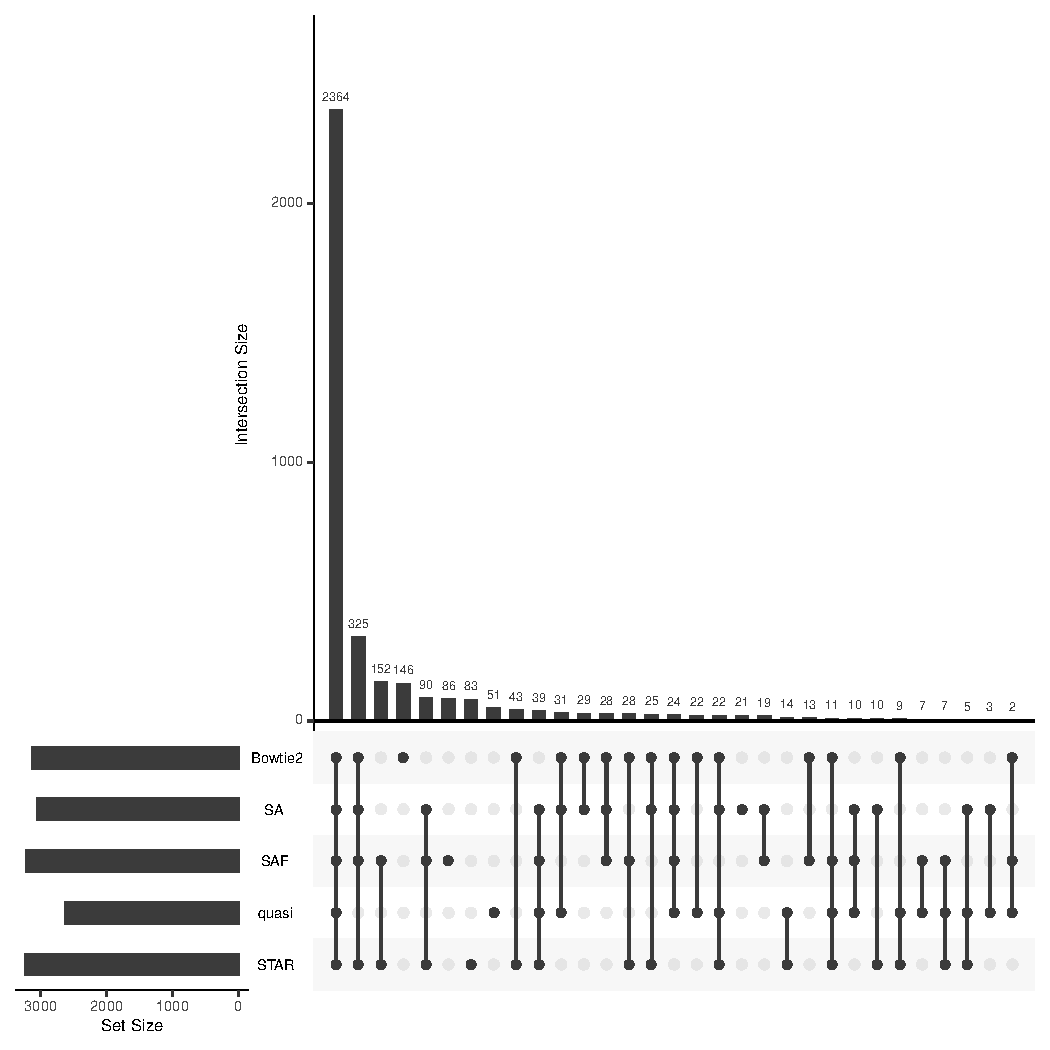
\includegraphics[width=\linewidth]{selal/zikafdr5.pdf}
		\caption{}
    \end{subfigure}
    ~ 
    \begin{subfigure}[t]{0.49\textwidth}
        \centering
  	  	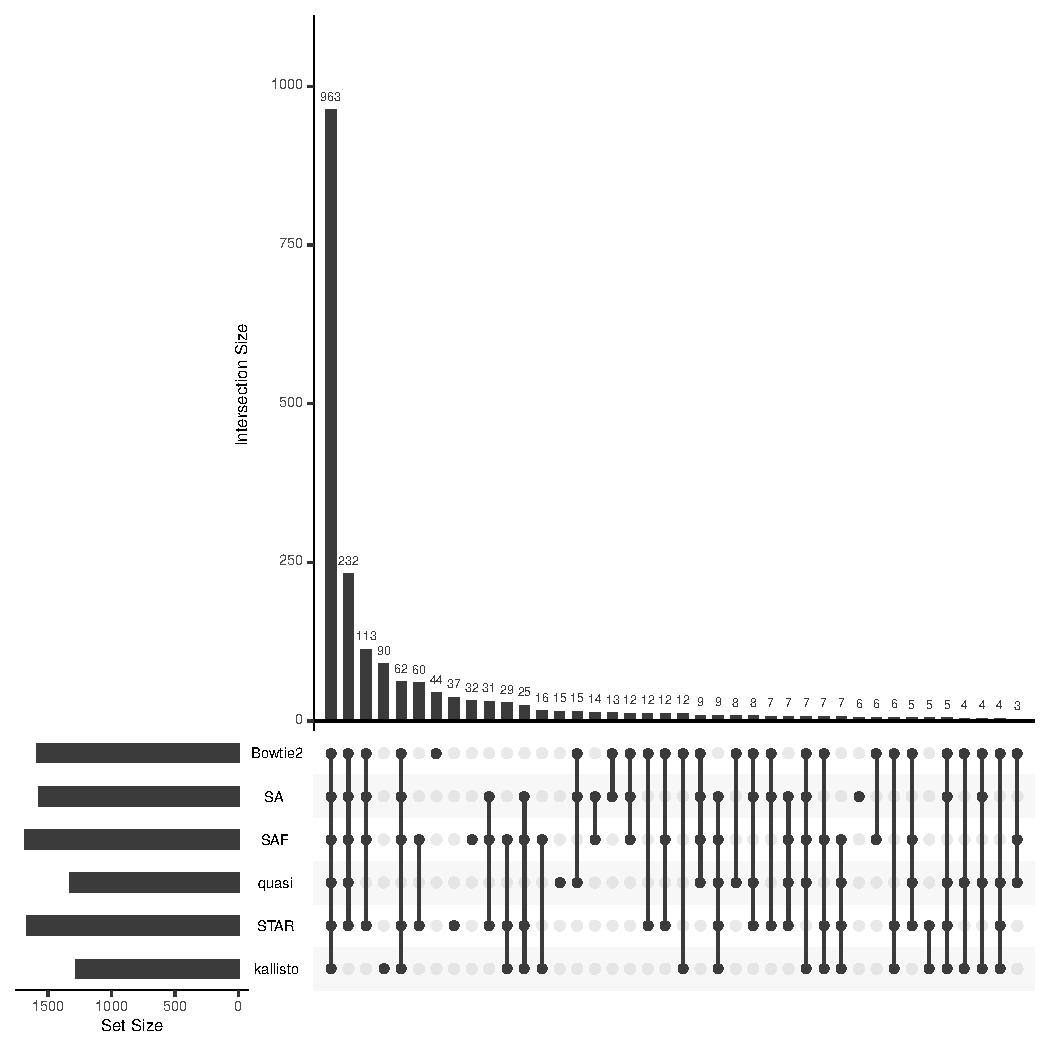
\includegraphics[width=\linewidth]{selal/zikakal.pdf}
		\caption{}
    \end{subfigure}
    \caption{Comparison of sets of differentially expressed transcripts, and their overlaps, computed using each method.
    Figure (a) shows the results when filtered at an FDR of $0.05$ and (b) shows the results at FDR $0.01$ after including kallisto as 
    an additional lightweight mapping approach.}
    \label{fig:suppdte}
\end{figure}